\documentclass[12pt]{article}

\usepackage[left=2.5cm,top=2.5cm,right=2.5cm,bottom=2.5cm]{geometry}
\usepackage{float}
\usepackage{graphicx}
\setlength{\parindent}{0pt}
\setlength{\parskip}{9pt}


\begin{document}
\title{COMP0005 Algorithms: Group Coursework Report}
\author{Group Number: 6}
\date{Academic year 2025/26}
\maketitle



\section{Experimental framework overview}

\subsection{Framework design and architecture}

All input data for testing are synthetically produced with the dedicated \texttt{TestDataGenerator} class as per the template provided. It produces random strings that are fixed to be both 10-character in length and lowercase alphabets. The total number of elements in the data pool is 110, 000, chosen to be slightly more than the largest checkpoint used, to ensure there is enough data for bulk insertions and timed measurement batches.

Three distinct data distributions are implemented for evaluation:

\begin{itemize}
    \item \textbf{Random}: Randomly generated strings serving as a baseline for other distributions and representing the quintessential unsorted input.
 
    \item \textbf{Sorted}: Strings generated in ascending lexicographical order, aimed to test the rebalancing mechanism of the trees as one of the worst-case inputs for the structures.
 
    \item \textbf{Reverse sorted}: Strings generated in descending lexicographical order intended to test the structures similar to the sorted distribution, representing worst-case inputs.
\end{itemize}
Each one of these data distributions are run through the framework separately and independently of one another.
Performance was measured and recorded at 11 distinct checkpoints:
\[
    [100, 250, 500, 1000, 2500, 5000, 10000, 25000, 50000, 75000, 100000]
\]
The insertion and search times of the algorithms are taken from the median of a batch of measurements across each of these checkpoints. The median was preferred over the mean as it reduces the effect of outliers produced by occasional timing spikes due to uncontrollable background OS processes. Results are demonstrated with a line graph using \texttt{matplotlib}.

\subsection{Hardware/software setup for experiments}
\begin{table}[H]
    \centering
    \begin{tabular}{|l|l|}
        \hline
        \textbf{Component} & \textbf{Specification} \\
        \hline
        Processor & AMD Ryzen 5 7535HS (6 cores, 12 threads, up to 4.55\,GHz) \\
        Memory    & 16\,GB RAM \\
        OS        & Windows 11 Home \\
        Language  & Python 3.14.3 \\
        Libraries & \texttt{timeit}, \texttt{random}, \texttt{string}, \texttt{matplotlib} \\
        \hline
    \end{tabular}
    \caption{Hardware and software specification of the test machine.}
    \label{tab:hw_sw}
\end{table}



\section{Performance results}


\subsection{Random Data Distribution}
Referring to the graph in Figure 1, the Left-Leaning Red-Black Tree (LLRB) consistently has the lowest insertion times among the three structures in results while the opposite is true for AVL tree which measured an approximate average insertion time of $1.1 \times 10^{-5}$ seconds at the final checkpoint of 100, 000 elements, compared to the LLRB and B Tree with an average insertion time of $0.8 \times 10^{-5}$ seconds and $0.9 \times 10^{-5}$ seconds respectively at the same checkpoint. Overall, all trees exhibit the expected $O (\log n)$ growth patterns with some irregularities due to noise.

The search operations on random input in Figure 2 show the LLRB tree to still be the fastest tree followed closely by the AVL tree, while the B Tree consistently ranks as the worst, measuring a time more than $3.0 \times 10^{-6}$ seconds at 100, 000 elements, which is more than double the measured times of the other two structures. The B Tree also shows irregularity that differs from other structures at around the 15000 element count mark, but the general upward trend still holds.

\begin{figure}[H]
    \centering
    \begin{minipage}{0.48\textwidth}
        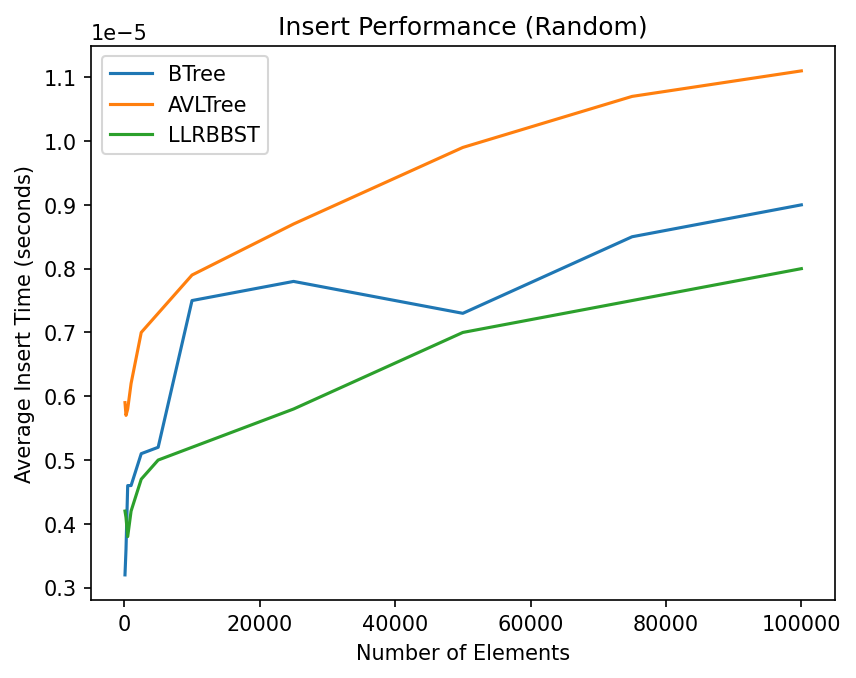
\includegraphics[width=\textwidth]{insert_performance_Random.png}
        \caption{Insert performance, random.}
    \end{minipage}
    \hfill
    \begin{minipage}{0.48\textwidth}
        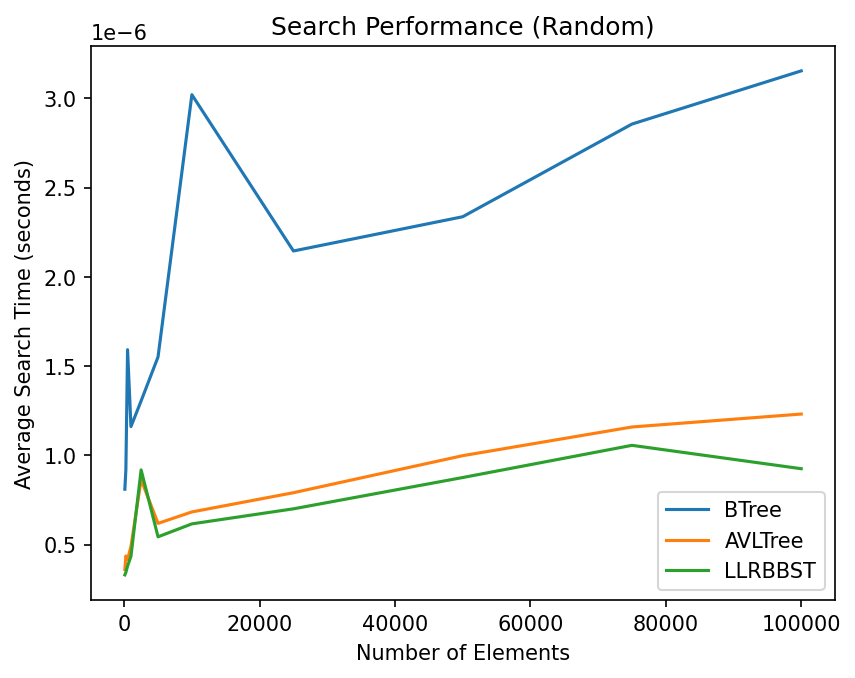
\includegraphics[width=\textwidth]{search_performance_Random.png}
        \caption{Search performance, random.}
    \end{minipage}
\end{figure}

\subsection{Sorted Data Distribution}
The results of insert operations under sorted inputs as shown in Figure 3 revealed the three structures having distinct time measurements with LLRB tree having the lowest time, followed by B Tree and the AVL tree respectively. Once again, irregularities appear in the curve for B Tree that differs from the other structures, but the trend still holds.

On the other hand, for the search operations in Figure 4 the average search times for the LLRB and AVL tree are very close to each other with both trees hovering around $1.0 \times 10^{-6}$ seconds. Additionally, the LLRB tree consistently has lower times until around the 90,000 element count mark, where the AVL tree surpasses it in speed. Similar to the search times for random inputs however, the B Tree still ranks as the worst structure.


\begin{figure}[H]
    \centering
    \begin{minipage}{0.48\textwidth}
        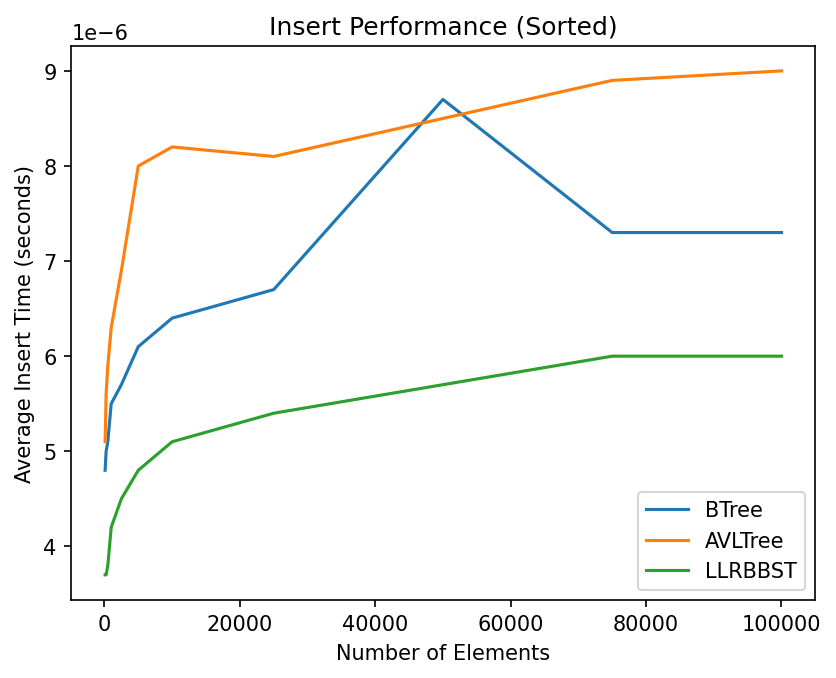
\includegraphics[width=\textwidth]{insert_performance_Sorted.png}
        \caption{Insert performance, sorted.}
    \end{minipage}
    \hfill
    \begin{minipage}{0.48\textwidth}
        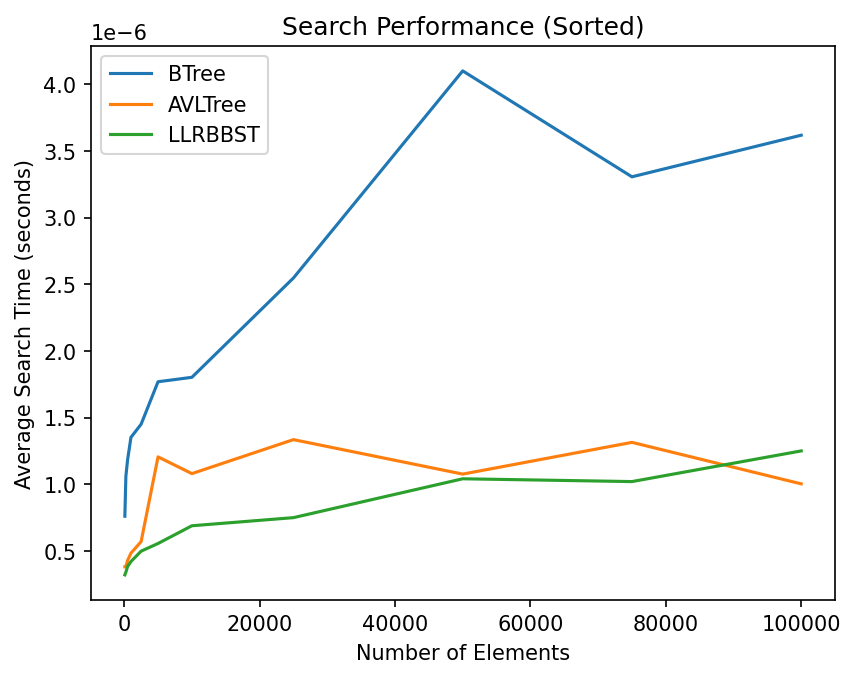
\includegraphics[width=\textwidth]{search_performance_Sorted.png}
        \caption{Search performance, sorted.}
    \end{minipage}
\end{figure}


\subsection{Reverse-sorted}

For insert operations, a large spike can be seen for the B Tree's graphs in Figure 5 around the 50, 000 element counts mark where it peaks at approximately $1.2 \times 10^{-5}$ seconds. Overall, the AVL tree consistently has the highest insertion times compared to the other two which hover around $0.6 \times 10^{-5}$ and $0.7 \times 10^{-5}$ seconds past the 10, 000 element counts.

Average search times under reverse-sorted inputs closely mirror the average search times under sorted inputs, which is expected as shown in Figure 6. LLRB tree generally has the lowest search times with the AVL tree following very closely with both measuring slightly more than $1.0 \times 10^{-6}$ seconds for 100, 000 elements. B Tree on the other hand, is significantly slower having an average search time of $4.0 \times 10^{-6}$ seconds at its peak at 50, 000 elements count (similar to sorted inputs) and just below $4.0 \times 10^{-6}$ seconds at 100, 000 element counts.



\begin{figure}[H]
    \centering
    \begin{minipage}{0.47\textwidth}
        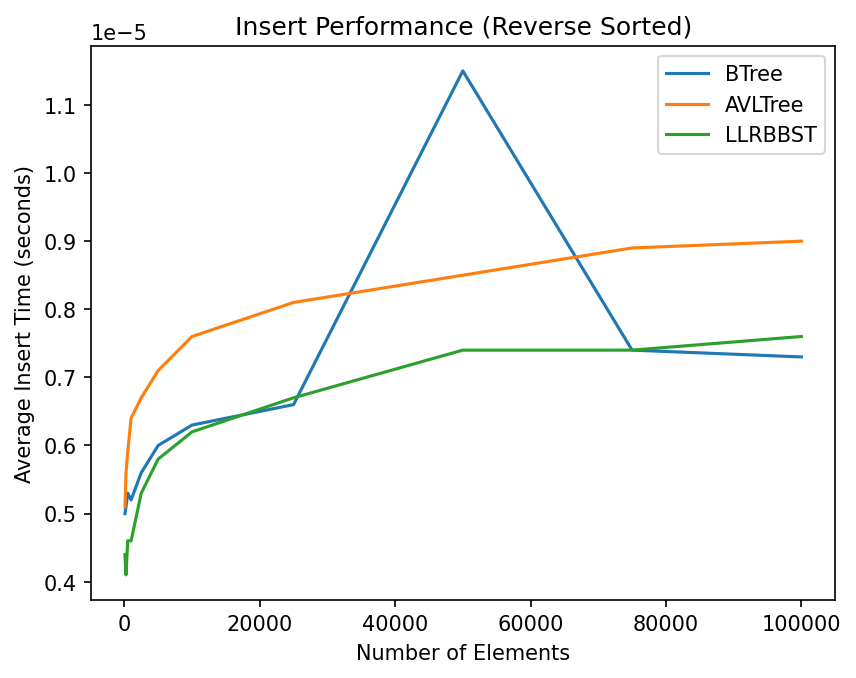
\includegraphics[width=\textwidth]{insert_performance_reverseSorted.png}
        \caption{Insert performance, reverse sorted.}
    \end{minipage}
    \hfill
    \begin{minipage}{0.47\textwidth}
        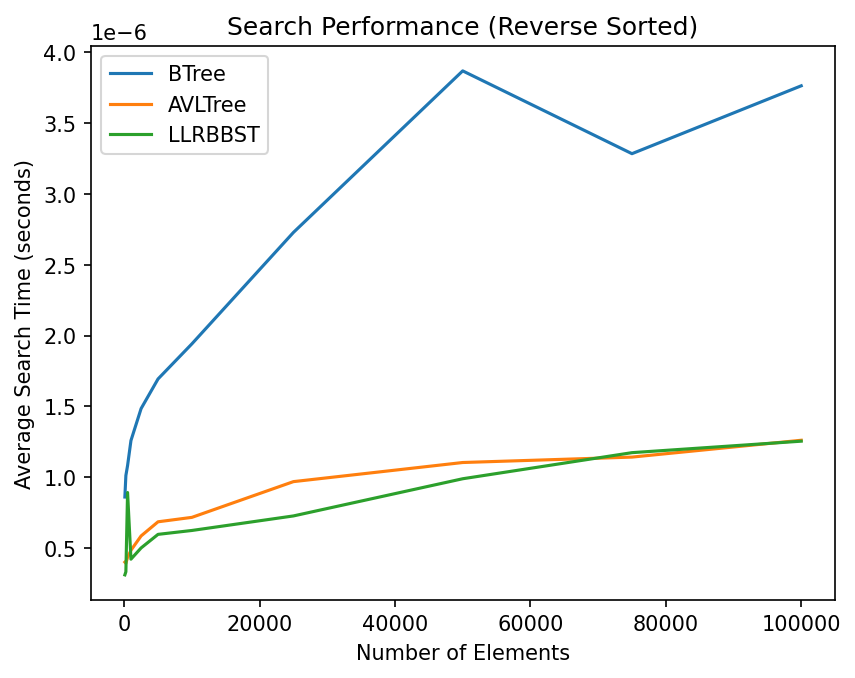
\includegraphics[width=\textwidth]{search_performance_reverseSorted.png}
        \caption{Search performance, reverse sorted.}
    \end{minipage}
\end{figure}



\section{Comparative assessment}
Based on the results and graphs, insert operations' performance are consistently topped by the LLRB tree, having the lowest average insertion times across the three data distributions. On the flipside, the AVL tree consistently performed the worst while the B Tree is overall in the middle despite having irregular spikes. The most prominent contributing factor towards the AVL tree's slow insertion time could be attributed to the fact that it checks for duplicates for every insert, which entails searching through the entire tree and adding $O(\log n)$ of cost which effectively doubles the work. The LLRB tree on the other hand checks for duplicates in its recursion process, making it more efficient. Overall however, all graphs closely show a trend of $O (\log n)$ growth which is expected of these data structures.

For search operations, the results differ from the inserts' performance where the B Tree consistently has the highest average measured time across all checkpoints, usually more than double the average time of the other two structures. This can be attributed to the fact that the B Tree needs to check for all keys that a node holds before descending to the next level, and with $t=2$, a node could hold up to 3 keys, but the tree's height would only be marginally smaller than the other two trees. This makes the traversal cost for the search operation on the B Tree much higher than the AVL and LLRB tree which execute only one check per level. The LLRB is again generally the fastest tree albeit marginally compared to the AVL tree which again may be attributable to its duplicate check being executed in the recursive descent rather than separately.

An important thing to address is also that the B Tree can be seen to be much more volatile compared to the others, which stems from its nature where the splitting of a node requires the redistribution of keys which may or may not propagate up multiple levels, and in worst-case all the way to the root, creating a new level. Since nodes hold different amounts of keys at different insertion points, it causes some inserts to be cheap while others are expensive, causing the volatility. This is especially true when the graph peaks which indicates a new level is created, and goes back down again.

Across different data distributions, the results are as expected, where the sorted and reverse-sorted inputs are generally faster, due to the rebalancing mechanism of these trees, which prevents the $O (n)$ height degeneration from occurring if it was a regular binary search tree.

Overall, the LLRB tree is consistently the fastest tree for insertions across the three distributions. The AVL tree while suffering from duplicate checks in insert operations performs similarly to the LLRB tree in searching making the AVL and LLRB trees the better choices for in-memory search-heavy processes rather than the B Tree. Despite poor performances within this experimental framework, in practical scenarios the B Tree is useful in processing large amounts of data in a node where $t$ is very large and utilizing disk-based storage to amortize the cost of scanning keys in a node by reading an entire node in a single operation~\cite{alma9931552389604761}. For an in-memory process with low values of $t$ as well as branching factors however, LLRB and AVL trees remain the better choices in terms of cost and time complexity.





\section{Team contributions}


\vspace{1cm}

\begin{tabular}{|l|l|p{6cm}|l|}
\hline
{\bf Name} & {\bf Portico ID} & {\bf Key contributions} & {\bf Work share (\%)} \\[1mm]
\hline
Arif    &  25125738  & Ran experiments, analyzed results and authored report & $25\%$ \\\hline
Yan     &25178418    &Developed experimentation framework, implemented BTree, reviewed report& $25\%$ \\\hline
          &            &         &          \\\hline
          &            &         &          \\
%% more entries as needed
\hline
\end{tabular}

\bibliographystyle{plain}
\bibliography{Primo_BibTeX_Export}
\end{document}
